\section{Das objektrelationale Modell}
\subsection{Einführung in objektrelationale Konzepte}
\begin{itemize}
	\item Vergleich ORDM zu RDM:
	\item Typen, Typkonstruktoren und ADT (statt nur Standard-Datentypen im RDM)
	\item Objektidentitäten (statt nur sichtbare, änderbare, lokale Schlüssel im RDM)
	\item Tabellen (geschachtelt und mit Objekten statt nur flach und mit Werten im RDM; statt Klassen im OODM-Sinne)
	\item Untertypen (Typhierarchie)
	\item Untertabellen (statt nur Fremdschlüssel im RDM, statt Klassenhierarchie im OODM-Sinne)
	\item Komponentenobjekte (statt nur Fremdschlüssel im RDM); Pfadausdrücke (statt vieler Verbunde im RDM)
	\item Anfragen und Sichten (analog zum RDM)
	\item Methoden (In SQL: UDMs) (statt nur Anwendungsprogramme auf Sichten im RDM)
\end{itemize}

\subsection{Der SQL:1999/SQL:2003 Standard}
\begin{itemize}
	\item \textbf{Objektrelationale Konzepte:}
	\item user defined types (UDTs)
	\item user defined functions (UDFs), User defined Methods (UDMs)
	\item Prozeduren, Funktionen, Methoden: Unterschiede bei Überladen und Overriding
	\item LOBs (Large Objects) und Locators für Laden von großen Daten bei effizienter Pufferausnutzung
	\item Typkonstruktoren (row, reference, array) (andere Collection-Konstruktoren: SQL:2003)\\
	row: Tupelkonstruktor\\
	array: einziger Collection Konstruktor\\
	reference: Komponentenobjekt
	\item Typ-, Tabellenhierarchien, Sichthierarchien (Object Views)
	
	\item \textbf{Conformance Level}
	\item SQL:1999 Kern ist\\
	SQL-92-Entry + einige Konzepte aus Transitional, Intermediate, Full Level + Kernkonzepte von SQL:1999-Foundation
	\item SQL:2003-Packages\\
	Enhanced Datetime Facilities\\
	Enhanced Integruty Management...\\
	Basic Object Support (eingeschränkte strukturierte und Referenz-Typen, Typkonzept, Typ-Test-Prädikate), LOB-Unterstützung mit Locators)\\
	Enhanced Object Support (alle Typkonstruktoren, Methoden, Tabellenhierarchie, Cast-Operatoren, Locators für komplexe Attributwerte)
\end{itemize}

\subsection{Der Strukturteil des ORDB-Modells}
\begin{itemize}
	\item \textbf{Typen}
	\begin{itemize}
		\item Standard-Datentypen
		\item Typkonstruktoren (unbenannte Typen)
		\item UDT: Datentyp \\
		Name, Repräsentation, Beziehung zu anderen Typen\\
		distinct types\\
		strukturierte (benannte) Tupeltypen: create type\\
		strukturierte (benannte) Objekttypen: create type
	\end{itemize}
	\item \textbf{Prozeduren, Funktionen, Methoden}
	\begin{itemize}
		\item UDF: Funktion (Methode, Prozedur)\\
		Name, Signatur, Resultat, Impl\\
		Prozedur: kein Überladen, statisches Binden\\
		Funktion: Überladen, statisches Binden\\
		Methoden: Überladen und Overriding, dynamisches Binden
	\end{itemize}
	
	\item \textbf{unbenannter Typkonstruktor row type}
	\begin{itemize}
		\item Tupeltyp hat keinen Namen, enthält Tupelwerte
		\item Tupeltyp als Wertebereich eines Attributs in einer Tabelle
		\item wird nur an dieser Stelle verwendet
		\item keine speziellen Funktionen, Methoden definierbar
		\begin{lstlisting}
		create table Personen	(PANr integer,
		Partner ref(Person),
		Wohnung row
			(PLZ integer, 
			Ort varchar(30),
			....
			)
		)
		\end{lstlisting}
	\end{itemize}
	
	\item \textbf{Unbenannter Typkonstruktor array type}
	\begin{itemize}
		\item einziger Collection Typkonstruktor in SQL:1999
		\item maximale Länge wie bei varchar mgl
		\item Operationen: Zugriff über Positionsnummer\\
		Kardinalität, Vergleich, Konstruktoren,...
		\begin{lstlisting}
		create table Personen	(PANr integer,
			Partner ref(Person),
			Wohnung row
				(PLZ integer, 
				Ort varchar(30),
				....
				)[4]
		)
		\end{lstlisting}
		eine Person kann bis zu 4 Personen haben
	\end{itemize}
	
	\item \textbf{Unbenannter Typkonstruktor multiset type}
	\begin{itemize}
		\item ab SQL:2003 Multimengen-(Bag)-Konstruktor
		\item Test, ob Multimenge eine Menge ist: is a set
		\item Multimenge $M_1$ in eine Menge umwandeln: set($M_1$)
		\item Element, Kardinalität, Teilmultimenge, Vereinigung, Durchschnitt, Differenz
			\begin{lstlisting}
			create table Personen	(PANr integer,
				Partner ref(Person),
					Wohnung row
					(PLZ integer, 
					Ort varchar(30),
					....
					) multiset
			)
			\end{lstlisting}
	\end{itemize}
	
	\item \textbf{UDT: Distinct Types}
	\begin{itemize}
		\item final: keine Untertypen definierbar
		\item definierbar: Vergleichsoperatoren, Casts, Methoden und Funktionen
		\begin{lstlisting}
		create type T1 as integer final
		create type T2 as integer final
		\end{lstlisting}
		erstellt zwei unvergleichbare Typen (zb Alter und Gewicht)
	\end{itemize}
	
	\item \textbf{UDT: strukturierter (benannter) Typ}
	\begin{itemize}
		\item können überall verwendet werden, auch als Parametertypen
		\item Persistenz: Konstruktorfuntkion Adresse() liefert Instanz des Typs (Default-Werte) oder insert
		\begin{lstlisting}
		create type Adresse as (PLZ, integer,...) not final
		\end{lstlisting}
		\begin{lstlisting}
		create type Person as (PANr integer, Partner ref(Person), Wohnung, Adresse,..)
		\end{lstlisting}
	\end{itemize}
	
	\item \textbf{UDTs: nicht-instantiierbar}
	\begin{itemize}
		\item virtuelle Typen: in OOPLs: abstrakte Klassen
		\item keine Instanzen definierbar
		\item nicht-instantiierbare Typen in SQL:2003
		\begin{lstlisting}
		create type T1 as (...)
			not instantiable not final
		\end{lstlisting}
	\end{itemize}
	
	\item \textbf{Typen als Attributtypen: UDTs und Typkonstruktoren}
	\begin{itemize}
		\item mit create type erzeugte Typen:
		\item können mit Methoden angereichert werden 
		\item können mit Untertypen verfeinert werden (falls not final)
		\item können als Attributtypen verwendet werden: Methoden sind dann auf Attribute anzuwenden
		\item können als Tabellentypen (Relationenschema) verwende werden: Methoden sind dann auf Objekte(oder Tupel) anzuwenden
		\\
		\\
		\item mit Typkonstruktoren row, array, multiset erzeugte Typen werden nur für Attribute eingesetzt
		\item keine Methoden und Untertypen definierbar
	\end{itemize}
	
	\item \textbf{UDTs: Tupeltypen und Objekttypen}
	\begin{itemize}
		\item mit create type erzeugte Typen:
		\item können Tupeltypen für Tabellen sein (relationale, evtl geschachtelte Tabelle ohne Objektidentitäten): Tabelle besteht aus (Tupel-)Werten
		\item können Objekttypen für Tabellen sein (Objekttabelle oder Objektrelation mit Objektidentitäten): Tabelle besteht aus (Tupel-)Objekten
		\item Beispiel: Tupeltyp
		\begin{lstlisting}
		create type Adresse as (PLZ integer, ...)
			not final;
		\end{lstlisting}
		\item Beispiel Objekttyp (durch Referenztypspezifikation)
		\begin{lstlisting}
		create type person as (PANr integer, Partner ref(Person), Wohnung Adresse,...)	
			not final
			ref is system generated;
		\end{lstlisting}
		\textit{Referenztypspezifikation von Objekttypen}
		\begin{itemize}
			\item ref is system generated\\
			Echte Objektidentität nach OODM, aber Eindeutigkeit nur in Tabelle
			\item ref from (Attributliste)\\
			etwa PANr, dann Objektidentität funktional bestimmt
			\item ref using Typ\\
			etwa integer, dann durch Benutzer zugewiesen
		\end{itemize}
		
	\end{itemize}
	
	\item \textbf{Untertypen}
	\begin{itemize}
		\item Einfach- oder Mehrfachvererbung(letzteres erst ab SQL4)
		\item Instantiierbarkeit und Abschluss
		\item nur Methoden dynamisch gebunden, nicht Funktionen
		\begin{lstlisting}
		create type Hiwi under Angestellter as (...)
			instantiable not final ...
		\end{lstlisting}
	\end{itemize}
	
	\item \textbf{Tabellen: Objektidentitäten}
	\begin{itemize}
		\item Typen ergänzen um OID => objektrelationale Tabellen
		\item objektrelationale Tabelle (auch Objekttabelle) ersetzt Begriff der Klasse, sie haben\\
		Objektidentitäten durch OIDs\\
		eine Extension (die Relation)\\
		einen Zustandstyp (mit of eingeleitet)
		\begin{lstlisting}
		create table Angestellte of Angestellter
			(ref is oid system generated)
		\end{lstlisting}
	\end{itemize}
	
	\item \textbf{Objektidentitäten und ihre Referenzgenerierungsart}
	\begin{itemize}
		\item Referenzgenerierungsart der Tabelle muss zu Referenztypspezifikation des Typs passen\\
		ref is name\_der\_oid-spalte system generated muss zu ref is system generated in Typ passen\\
		ref is name\_der\_oid-spalte derived muss zu ref from (Attributliste) in Typ passen\\
		ref is name\_der\_oid-spalte user generated muss zu ref using Typ in Typ passen
		\item bei derived muss Attributliste primary key oder (unique und not null) sein
		\item Die oid-Spalte hat dann folgenden Typ:\\
		\textit{ref(Typname)scope(Tabellename)}
		\item abstrakte Domäne der Objektidentität ist für den Typ spezifiziert
		\item die aktuelle Objektmenge (Extension) wird durch scope auf die aktuell in der Tabelle vorhandenen OIDs eingeschränkt
	\end{itemize}
	
	\item parallel zur Typhierarchie mit under auch \textbf{Tabellenhierarchien}
	\begin{itemize}
		\item aufgrund der Isomorphie von Typ- und Tabellenhierarchie auch hier nur Einfachvererbung erlaubt
		\item Untertabelle ist Teilmenge der Obertabelle (projiziert auf die Spalten der Obertabelle)
		\item Untertabelle kann nichtredundant /redundant definiert bzw gespeichert werden:\\
		nichtredundant, split instance\\
		redundant, repeat class
	\end{itemize}
\end{itemize}


\subsection{Der Operationenteil des ORDB-Modells}
\begin{itemize}
	\item \textbf{Die SFW-Klausel im objektrelationalen SQL}
	\begin{itemize}
		\item strukturidentisch mit SQL: SELECT FROM WHERE GROUP BY HAVING
		\item und Aggregatfunktionen, Sortierung, Umbenennung, Mengenoperationen, Verbundoperationen,.. auch vom relationalen SQL
		\item zusätzlich: tiefe vs. flache Extension\\
		navigierende Anfragen (Pfadausdrücke)\\
		Anfragen mit Methodenaufrufen\\
		typspezifische Anfragen (etwa mit Collection-Attributen)
		
		\item Anfragen an Tabelle auch an Untertabelle\\
		select ... from Angestellte...\\
		liefert auch Hiwis
		\item Einschränkungen der Substituierbarkeit mgl
		\item Pfadausdrücke für Komponentenobjekte:\\
		Referenzen mit scope verwendbar; Methoden; Dereferenzieren liefert Objekt mit Zustand
	\end{itemize}
	\item \textbf{Object Views: Sichthierarchien}
	\begin{itemize}
		\item objekterhaltende Sichten
		\begin{lstlisting}
		create view Keine_Hiwis of Angestellter
			as select ... from only (Angestellte)
		\end{lstlisting}
		\item abgeleitete Sichten auf referenzierten (Komponenten-)Tabellen:
		\item Anfrageergebnisse können dynamisch in neuen Sichthierarchien eingeordnet werden
		\item letzteres verwirklicht dynamische Typisierung und Klassifizierung \textit{per Hand}
	\end{itemize}
\end{itemize}


\subsection{Höhere Konzepte des ORDB-Modells}
\begin{itemize}
	\item \textbf{Methoden und Konstruktoren}
	\begin{lstlisting}
	create type Angestellter as
		(Basisgehalt decimal(9,2),
		...)
		instantiable not final
		method Endgehalt()
			returns decimal (9,2);
	\end{lstlisting}
	\begin{lstlisting}
	create method Endgehalt() for Angestellter
		<Methodenrumpf>;
	\end{lstlisting}
	\begin{lstlisting}
	create type Hiwi under Angestellter as
		(...)
		instantiable not final
		overriding method Endgehalt()
			reutnrs decimal(9,2);
	\end{lstlisting}
	
	Konstruktorfunktion \textit{Adresse()} liefert Instanz des Typs (Default-Werte) oder insert
	
	\item \textbf{UDF: Methodendefinition}
	\begin{itemize}
		\item Methoden sind Funktionen, die  an einen UDT gebunden sind
		\item impliziter self-Parameter, Signatur und Impl getrennt
		\item Signaturen müssen identisch sein\\
		No-Varianz (statt Ko- und Kontravarianz)\\
		kein multple dynamic dispatch
		
		\item Methodenaufruf mit Dot-Notation
	\end{itemize}
\end{itemize}

\begin{figure}[!h]
	\centering
	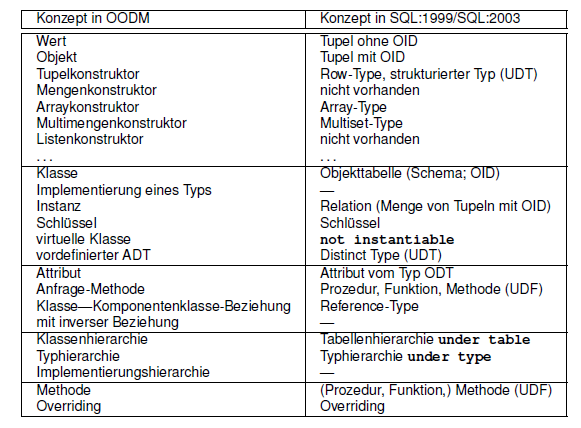
\includegraphics[scale=0.6]{img/ordb_modell_summary.png}
	\caption{Zusammenfassender Vergleich OODM und Standard Konzepte}
\end{figure}

\newpage
\subsection{Umsetzung in ORDBMS}
\begin{itemize}
	\item fehlende Umsetzung in ORDBMS: viele Teile des Standards fehlen bzw. sind abweichend davon umgesetzt
	\item Typkonstruktoren kaum vorhanden und nicht orthogonal umgesetzt
	\item Klassen- und Typhierarchie teilweise nur eine von beiden umgesetzt
	\item Objektidentitäten: nicht alle drei Optionen der Referenzgenerierung umgesetzt\\
	....
\end{itemize}


\subsection{Fazit und Vergleich}
\begin{itemize}
	\item \textbf{Modellierung - das Manta-Problem}
	\begin{itemize}
		\item Rollen, Rollenwechsel, Mehrfachzugehörigkeit von Objekten zu Klassen
		\item Typ- und Klassenhierarchie (wie OODM, ORDM)
	\end{itemize}
	
	\item \textbf{Sichten - das Manta-Problem}
	\begin{itemize}
		\item Klassen durch Anfragen und zusätzliche Strukturdefinitionen dynamisch ableiten
		\item diese Sichtklassen wie Basisklassen nutzbar machen
	\end{itemize}
	
	\item \textbf{Datenunabhängigkeit - das Fahrrad-Problem}
	\begin{itemize}
		\item Drei Ebenen Konzept gilt fü DBMS, nicht für RDBMS
		\item je nach Anwendungssituation, flexible Speicherstrukturen intern ermöglichen
	\end{itemize}
	\item impedance mismatch mindern
	\item Persistenz: Extension und Fortpflanzung
	\item \textbf{Mehrfachzugehörigkeit von Klassen}
	\begin{itemize}
		\item keine Lösung (in OODBPL): Rollenobjekte als Komponente jedem Objekt mitgeben\\
		Nachteile: Objekte und ihre ROllen bilden dann keine Klassen- und Typhierarchie\\
		Rollen erweitern dann nicht den Typ\\
		Vererbung und Overriding dann nicht nutzbar\\
		so simulieren kann man es auch relational
		
		\item keine Lösung (in OODBPL und manchen ORDBMS)\\
		tiefe Extension simuliert Mehrfachzugehörigkeit\\
		aber kein allgemeines Inklusionsprinzip (disjunkter Durchschnitt)\\
		Objekte werden immer in speziellster Klasse erzeugt
	\end{itemize}
	
	\item \textbf{Manta-Problem}
	\begin{figure}[!h]
		\centering
		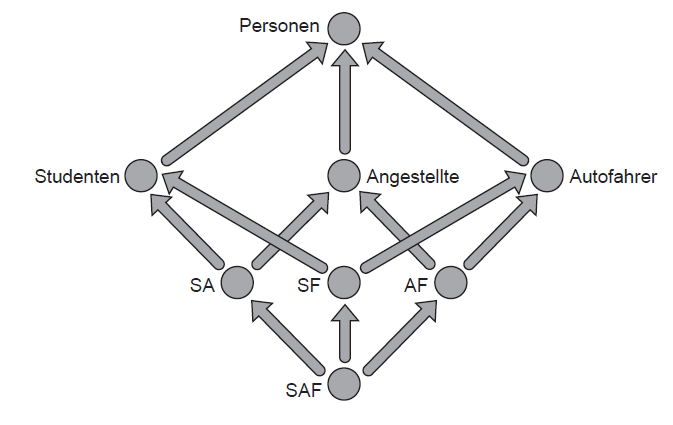
\includegraphics[scale=0.5]{img/mantra_problem_ex.png}
		\caption{Mantra Problem Beispiel}
	\end{figure}\\
	Lösung:
	\begin{itemize}
		\item im Schema Klasse K definieren
		\item mit klassenbasierten Anfragen definiert man dynamisch die Unterklassen
		\item in diesen Sichtklassen wird dann die von Klasse K vererbten Methoden jeweils geeignet redefiniert
		\item Falls Objekt in mehreren Klassen, dann Konfliktauflösemethode spezifizieren
	\end{itemize}
	
	\item \textbf{Einschänkungen ODMG} siehe \ref{odmg_constraints}
	
	\item \textbf{Einschränkungen SQL:2003}
	\begin{itemize}
		\item Standard nicht vollständig \\
		Bsp: Typkonstruktoren schrittweise eingeführt und nicht orthogonal
		\item Klassen und Typhierarchie müssen isomorph (bijektiv - eineindeutig) sein
		\item impedance mismatch: Objekttabellen und Java-Klassen
		\item keine persistente Programmierumgebung nach Atkinson (siehe Kap 5)
		\item Mehrfachvererbung nicht vorhanden
		\item Anfragen nur extensionsbasiert
	\end{itemize}
\end{itemize}